\documentclass[10pt]{article}
\usepackage[margin=0.90in]{geometry}
\usepackage{amsmath,amssymb,amsthm,mathtools}
\usepackage{microtype}
\usepackage{graphicx}
\usepackage[hidelinks]{hyperref}
\usepackage{fontawesome5}
\usepackage{enumitem}
\usepackage{indentfirst}
\usepackage[most]{tcolorbox}
\setlist{leftmargin=1.15em,itemsep=0.15em,topsep=0.25em}
\setlength{\parindent}{1.5em}
\setlength{\parskip}{0.10em}
\setlength{\textfloatsep}{0.8em}

\definecolor{conceptblue}{HTML}{315F86}
\definecolor{conceptink}{HTML}{263746}
\definecolor{conceptback}{HTML}{F3F7FA}
\newtcolorbox{conceptbox}{
  enhanced,
  breakable,
  colback=conceptback,
  colframe=conceptblue,
  colbacktitle=conceptback,
  coltitle=conceptblue,
  boxrule=0pt,
  borderline west={2.2pt}{0pt}{conceptblue},
  arc=1.5mm,
  left=0.85em,
  right=0.85em,
  top=0.45em,
  bottom=0.35em,
  before skip=0.45em,
  after skip=0.65em,
  title={Conceptual Interpretation},
  fonttitle=\sffamily\bfseries\small,
  fontupper=\sffamily\small\color{conceptink},
}

\newtheorem{proposition}{Proposition}
\newtheorem{definition}{Definition}

\begin{document}

\begin{center}
{\LARGE \bfseries The Physics Response Spectrum of Recursive LLMs\par}
\vspace{0.15em}
{\large Collapse, churn, and takeoff under one selection law\par}
\vspace{0.75em}
{\large Jonathan R. Landers\par}
\vspace{0.25em}
{July 2026\par}
\vspace{0.15em}
{\small\href{https://github.com/jonland82/finite-response-kernels}{\faGithub\ Project Repository}\par}
\end{center}

\vspace{0.35em}

\begin{abstract}
Recursive revision is often discussed as if repetition itself determined the outcome. We make its direction a controlled variable. Fixed-weight Amazon Nova Lite solves 31 difficult PHYBench problems in populations of four, revises selected solutions for six rounds, and resamples children with pressure $\rho\in\{-6,-2,0,2,6\}$. One scalar law produces a statistically resolved spectrum: mean expression fitness falls from $0.0749$ to $0.0257$ at $\rho=-6$, remains near baseline at $\rho=0$, and rises to $0.1939$ at $\rho=2$. Exact population accuracy independently rises from $1.21\%$ to $8.87\%$. A signed takeoff kernel records when response arrives; total response separates monotone gain from churn. Matched restart and frozen-context controls show that selection alone helps, while inherited revision amplifies the positive branch. Selection supplies direction, recursion mediates it, and takeoff is the finite response of their composition.
\end{abstract}

\section{One loop, three outcomes}

\begin{conceptbox}
\begin{itemize}[leftmargin=1.15em,itemsep=0.18em,topsep=0.05em]
\item Recursion is an amplifier, not a direction. Selection pressure determines whether repeated revision drives deterioration, churn, or improvement.
\item A nearly unchanged endpoint can hide substantial internal motion. Neutral response means little net gain, not necessarily a static population.
\item Takeoff is best understood as a trajectory delivered across several rounds, rather than as one sudden jump.
\end{itemize}
\end{conceptbox}

A model generates answers, a rule selects survivors, and the survivors become the next prompt. This loop is frequently described by its hoped-for endpoint of self-improvement or its feared endpoint of model collapse. Neither endpoint follows from recursion alone. Recursive synthetic data can contract a distribution, while filtering and retained real data can stabilize or improve it \cite{shumailov2024,kazdan2025}. The missing object is a controlled response curve connecting the regimes.

We construct that curve on physics reasoning. The model weights, prompt family, population size, and problems remain fixed. Only a scalar selection pressure $\rho$ changes. Negative $\rho$ favors weak solutions, $\rho=0$ is score-blind propagation, and positive $\rho$ favors strong solutions. The experiment therefore asks a sharper question than ``does self-revision work?'': how does a recursive solution population respond as selection is continuously turned from adversarial to constructive?

The answer is an ordered dynamical spectrum. Strong negative selection produces nearly monotone collapse. Neutral selection produces small terminal motion with substantial internal churn. Positive selection produces rapid improvement in both a continuous symbolic score and exact answers. The transition is steepest between $\rho=0$ and $\rho=2$.

This also realizes the source-kernel separation of finite response \cite{landersEntropy}. Selection is the oriented source: it injects pressure toward or away from good answers. Recursive revision is the mediator: it distributes that pressure across rounds. What is observed is not an instantaneous jump but a finite takeoff kernel.

\section{A calibrated recursive experiment}

\begin{conceptbox}
\begin{itemize}[leftmargin=1.15em,itemsep=0.18em,topsep=0.05em]
\item Each problem carries a four-answer population. The model revises every answer, then selection resamples the children that seed the next round.
\item The parameter $\rho$ changes survival odds without changing model weights or revealing the gold answer. Paired initial populations isolate this selection effect.
\item Fitness variation is the fuel for response: the selector's local sensitivity is exactly the score variance available in the child pool.
\end{itemize}
\end{conceptbox}

\textbf{Problems and model.} PHYBench is a curated benchmark of multi-step physical reasoning with symbolic answers and an expression-aware score \cite{qiu2025}. We began from its 100 fully annotated text problems. A deterministic parser gate retained 78; stratified splitting assigned 16 to calibration, 31 to the reported spectrum, and 31 to a locked set. The spectrum contains 13 mechanics, 10 electricity, four thermodynamics, two optics, one modern-physics, and one advanced-physics problem.

Amazon Nova Lite \cite{amazonNova} was called through Bedrock with fixed weights, temperature $0.8$, top-$p$ $0.9$, and at most 900 output tokens. Required tool output contained a derivation, one final expression, and a unit. Nova saw the problem and one inherited attempt, but never the gold answer, fitness, selector, or value of $\rho$.

\textbf{Population dynamics.} For problem $p$ and replicate $j$, four independent calls form the shared round-zero population
\[
X_{pj0}=(x_{pj01},\ldots,x_{pj04}).
\]
At round $r+1$, each parent produces one revised child through the stochastic generator $\mathcal G$,
\[
y_{pj,r+1,i}\sim\mathcal G(\text{problem}_p,x_{pjri}),\qquad i=1,\ldots,4.
\]
Parents never survive directly. Resampling four children with replacement forms $X_{pj,r+1}$ and permits concentration or recovery. All five $\rho$ conditions share the same $X_{pj0}$ within a replicate; there are two replicates and six recursive rounds.

\textbf{Fitness and exact correctness.} Let $C(x)\in\{0,1\}$ denote exact symbolic equivalence. Because exact answers were sparse, PHYBench's Expression Edit Distance (EED) supplies selection fitness $s(x)\in[0,1]$ while $C$ remains an independent outcome. For tree distance $d$ from a gold tree of size $L$,
\begin{equation}\label{eq:eed}
s(x)=\max\!\left(0,0.6-\frac{d}{L}\right),
\qquad s(x)=1\ \text{for an exact symbolic match}.
\end{equation}
Unparseable expressions receive zero; 91.1\% of primary expressions parsed successfully.

\textbf{One selection law.} Given the four child scores $s_1,\ldots,s_4$,
\begin{equation}\label{eq:selection}
p_i(\rho)=\frac{\exp[\rho(s_i-\tfrac12)]}
{\sum_{\ell=1}^{4}\exp[\rho(s_\ell-\tfrac12)]},
\qquad (N_1,\ldots,N_4)\sim\operatorname{Multinomial}(4;p_1,\ldots,p_4).
\end{equation}
Child $i$ appears $N_i$ times in the next population.

\begin{proposition}[Selection susceptibility]\label{prop:selector}
For a fixed child pool, let $\bar s(\rho)=\sum_i p_i(\rho)s_i$ be expected selected fitness. Then
\begin{equation}\label{eq:variance-response}
\frac{d\bar s}{d\rho}=\operatorname{Var}_{p_\rho}(s)\ge0.
\end{equation}
Selection is strictly responsive exactly when the child pool contains fitness variation.
\end{proposition}

\begin{proof}
Differentiate the softmax: $\partial_\rho p_i=p_i(s_i-\bar s)$. Multiplication by $s_i$ and summation give Eq.~\eqref{eq:variance-response}.
\end{proof}

Thus $\rho$ is calibrated within every child pool. Across rounds the selected population changes the next pool, allowing thresholds, saturation, and path dependence.

\clearpage
\section{Takeoff as finite response}

\begin{conceptbox}
\begin{itemize}[leftmargin=1.15em,itemsep=0.18em,topsep=0.05em]
\item Terminal gain $g$ says where the process finishes, while total response $A$ says how much movement occurred along the way.
\item The gap $E=A-|g|$ measures motion erased by reversal. The two cone boundaries are coherent collapse and coherent takeoff; the interior records churn.
\item The Markov-kernel expansion shows why timing matters: pressure introduced at any round can propagate through every later revision stage.
\end{itemize}
\end{conceptbox}

Let
\begin{equation}\label{eq:population-score}
q_{pjr}(\rho)=\frac14\sum_{i=1}^{4}s(x_{pjri}),
\qquad
Q_r(\rho)=\frac{1}{62}\sum_{p=1}^{31}\sum_{j=1}^{2}q_{pjr}(\rho).
\end{equation}
Write the roundwise response, terminal gain, and total response as
\begin{equation}\label{eq:response}
\Delta_r=Q_r-Q_{r-1},\qquad
g=Q_6-Q_0,\qquad
A=\sum_{r=1}^{6}|\Delta_r|.
\end{equation}
When $g\ne0$, the signed normalized takeoff kernel is
\begin{equation}\label{eq:takeoff-kernel}
\kappa_r=\frac{\Delta_r}{|g|},
\qquad \sum_{r=1}^{6}\kappa_r=\operatorname{sign}(g).
\end{equation}
It records not merely whether the population improves, but when the improvement arrives. The finite-response geometry follows from the triangle inequality,
\begin{equation}\label{eq:wall}
A\ge |g|,\qquad E=A-|g|\ge0.
\end{equation}
The admissible trajectories form the response cone $\mathcal C=\{(g,A):A\ge |g|\}$. Its left boundary $A=-g$ is monotone collapse, its right boundary $A=g$ is monotone takeoff, and its vertical interior near $g=0$ is neutral churn. Height $E$ above the boundary is response erased by reversal. This is the discrete takeoff analogue of the sharp boundary and broadened interior in causal kernel space \cite{landersEntropy}: a one-round jump is delta-like, a distributed monotone trajectory is mediated response, and an interior trajectory carries ringing or churn.

At the transition-law level, recursive prompting is a Markov kernel $P_\rho$ on solution populations. With initial distribution $\mu_0$ and score vector $Q$,
\begin{equation}\label{eq:duhamel}
q_r(\rho)=\mu_0P_\rho^rQ,
\qquad
\partial_\rho q_r
=\sum_{u=0}^{r-1}\mu_0P_\rho^u(\partial_\rho P_\rho)P_\rho^{r-1-u}Q.
\end{equation}
Equation~\eqref{eq:duhamel} is the discrete finite-response formula: a change in selection can enter at any stage $u$ and propagate through every later revision. Its roundwise difference is the tangent takeoff kernel.

\begin{figure}[t]
\centering
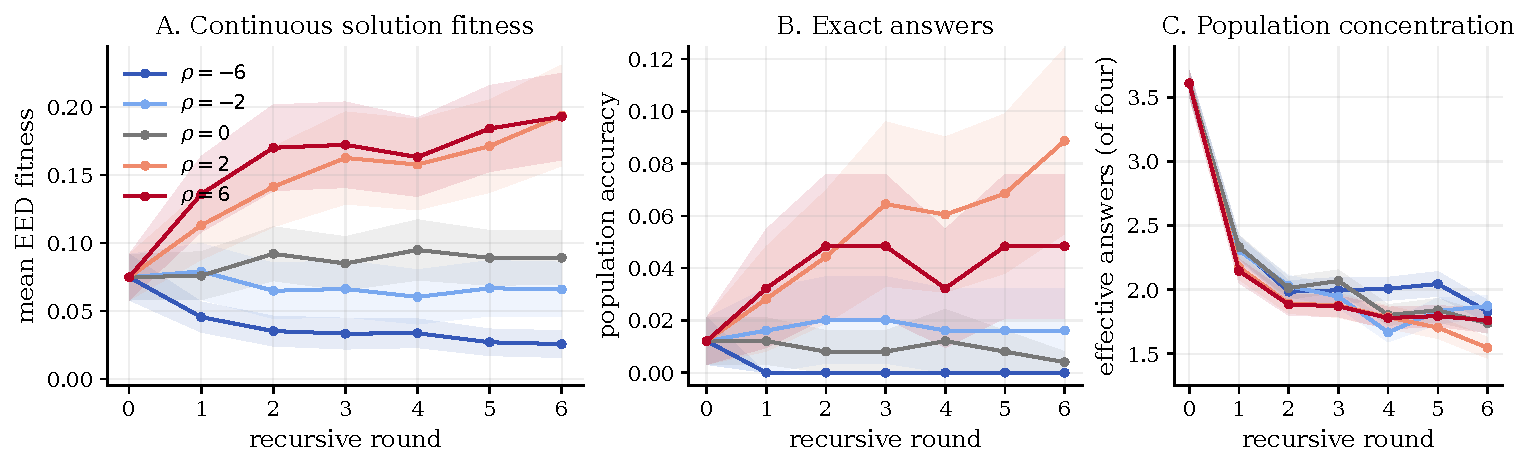
\includegraphics[width=0.99\linewidth]{fig1_physics_response_spectrum.pdf}
\caption{One fixed model, one selection law, three regimes. \textbf{A}: mean EED fitness over 31 problems and two paired replicates. \textbf{B}: exact population accuracy independently follows the positive branch. \textbf{C}: every branch concentrates, but $\rho=2$ produces the strongest takeover of the four-slot population. Shading is $\pm1$ standard error over 62 problem-replicate units.}
\label{fig:primary}
\end{figure}

\section{The empirical response spectrum}

\begin{conceptbox}
\begin{itemize}[leftmargin=1.15em,itemsep=0.18em,topsep=0.05em]
\item The same recursive system exhibits three resolved regimes: collapse at strong negative pressure, churn near zero, and takeoff under positive pressure.
\item Exact symbolic answers corroborate the continuous score. Moderate positive pressure at $\rho=2$ outperforms the more aggressive $\rho=6$ condition on exact accuracy.
\item Population concentration and solution quality are separate axes. A lineage can take over while carrying either weak or strong answers.
\end{itemize}
\end{conceptbox}

Figure~\ref{fig:primary} shows immediate separation. Every condition begins at $Q_0=0.0749$. Negative selection drives the population to $0.0257$. Score-blind propagation ends at $0.0892$. Positive selection reaches $0.1939$ at $\rho=2$ and $0.1930$ at $\rho=6$.

\begin{center}
\small
\begin{tabular}{rrrrrr}
\hline
$\rho$ & $Q_6$ & $g$ & $A$ & exact at $r=6$ & distinct fraction\\
\hline
$-6$ & 0.0257 & $-0.0492$ & 0.0498 & 0.00\% & 0.500\\
$-2$ & 0.0659 & $-0.0090$ & 0.0329 & 1.61\% & 0.520\\
$0$  & 0.0892 & $+0.0143$ & 0.0403 & 0.40\% & 0.476\\
$2$  & 0.1939 & $+0.1190$ & 0.1288 & 8.87\% & 0.423\\
$6$  & 0.1930 & $+0.1181$ & 0.1364 & 4.84\% & 0.480\\
\hline
\end{tabular}
\end{center}

The collapse and improvement branches are statistically resolved when problems are bootstrapped as the independent units. The $\rho=-6$ endpoint gain has 95\% interval $[-0.0894,-0.0163]$; $\rho=2$ has $[0.0510,0.2014]$; and $\rho=6$ has $[0.0669,0.1772]$. Relative to neutral selection, terminal EED differs by $-0.0636$, $+0.1047$, and $+0.1038$ for $\rho=-6,2,6$, respectively, with all three intervals excluding zero.

Exact correctness corroborates the continuous metric. Round zero contains three correct survivor slots from one problem. At $\rho=2$, round six contains 22 correct slots spanning four problems, and exact accuracy gains $0.0766$ with 95\% interval $[0.0081,0.1653]$. Stronger selection is not uniformly better: $\rho=6$ has the same EED plateau but only 12 correct terminal slots. Moderate positive pressure found the best balance between retaining strong answers and continuing to explore.

The path geometry distinguishes the regimes. At $\rho=-6$, $E=A-|g|=0.0006$: collapse is almost monotone. At $\rho=2$, $E=0.0098$: most positive response survives. Neutral selection has only $g=0.0143$ but $A=0.0403$, so nearly two thirds of its motion is erased. Neutrality here is churn, not stasis.

Selection also concentrates populations. The effective number of answers falls from $3.61$ of four at round zero to $1.55$ at $\rho=2$. This is not merely collapse: concentration can preserve a winning lineage and raise accuracy. Diversity loss and quality loss are separate axes.

Electricity supplies the strongest positive response: at $\rho=2$ its EED gain is $0.2257$ and exact accuracy reaches 25\%. Mechanics gains $0.0724$ without an exact terminal answer; thermodynamics gains $0.0617$ and reaches 6.25\% exact. The spectrum is therefore broad, while exact takeoff begins in domains where the generator can already produce rare correct variants.

\section{What recursive inheritance adds}

\begin{conceptbox}
\begin{itemize}[leftmargin=1.15em,itemsep=0.18em,topsep=0.05em]
\item Restart controls show that repeated generation plus selection can improve performance even without inherited attempts.
\item Recursive context adds stateful repair. It lets later generations preserve, inspect, and revise what earlier generations discovered.
\item Inheritance amplifies the selector's direction in both signs. The same memory channel strengthens constructive improvement and destructive collapse.
\end{itemize}
\end{conceptbox}

To separate inheritance from repeated sampling, we reused the identical round-zero populations for eight problems and compared three channels at $\rho\in\{-6,0,2\}$. Recursive children saw the selected parent; restart children saw only the problem; frozen children always saw their assigned round-zero attempt. All other settings and the selector were unchanged.

\begin{figure}[t]
\centering
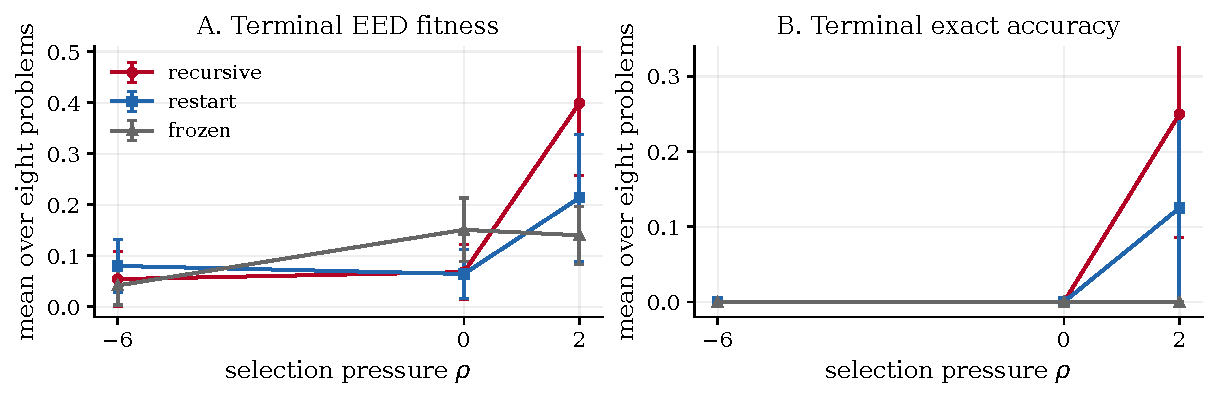
\includegraphics[width=0.90\linewidth]{fig2_context_controls.pdf}
\caption{Matched context controls on eight problems. Recursive inheritance produces the strongest positive branch: at $\rho=2$, terminal EED is $0.399$ under recursion, $0.214$ under restart, and $0.140$ under frozen context; exact accuracy is 25\%, 12.5\%, and 0\%. Error bars are $\pm1$ standard error over problems.}
\label{fig:controls}
\end{figure}

Restart improves at $\rho=2$, proving that repeated fresh generation plus selection already has power. Recursion then amplifies it. On the matched subset, recursive terminal EED exceeds restart by $0.185$ and frozen context by $0.259$. The latter paired problem-bootstrap interval is $[0.051,0.515]$. Recursive exact accuracy doubles restart and exceeds frozen by 25 percentage points. The productive mechanism is therefore layered: generation supplies variation, selection retains it, and inherited revision compounds it.

The negative branch compounds too. Recursive $\rho=-6$ loses $0.0496$ EED on the subset. The same channel that sharpens constructive selection transmits destructive selection. Recursion is an amplifier with sign supplied by the selector.

\section{Takeoff is a response, not a moment}

\begin{conceptbox}
\begin{itemize}[leftmargin=1.15em,itemsep=0.18em,topsep=0.05em]
\item A convincing takeoff combines positive terminal gain, high response efficiency, and a positive inheritance lift over restart.
\item The $\rho=2$ branch is distributed across rounds and largely retained. Its endpoint is the accumulated output of the recursive channel, not a lucky final sample.
\item Fixed model weights already expose a controllable inference-time takeoff kernel. Weight updates would add a second, slower adaptive layer.
\end{itemize}
\end{conceptbox}

This experiment turns takeoff from a metaphor into a measured finite-response object. The scalar $g$ identifies direction and magnitude. The kernel $\kappa$ identifies delivery across rounds. The pair $(g,A)$ locates each trajectory inside the response cone. Selection susceptibility explains why a diverse child pool can respond sharply, while Eq.~\eqref{eq:duhamel} shows how that local tilt propagates through a recursive cascade.

The result is strongest at $\rho=2$: large terminal displacement, little erased response, a rising exact-answer curve, and a clear advantage for inherited revision over frozen context. The nearly equal EED endpoints at $\rho=2$ and $6$, together with higher exact accuracy at $2$, also show that takeoff is not synonymous with maximal pressure. A selector must preserve enough variation for the generator to discover and repair.

\clearpage
\begin{figure}[t]
\centering
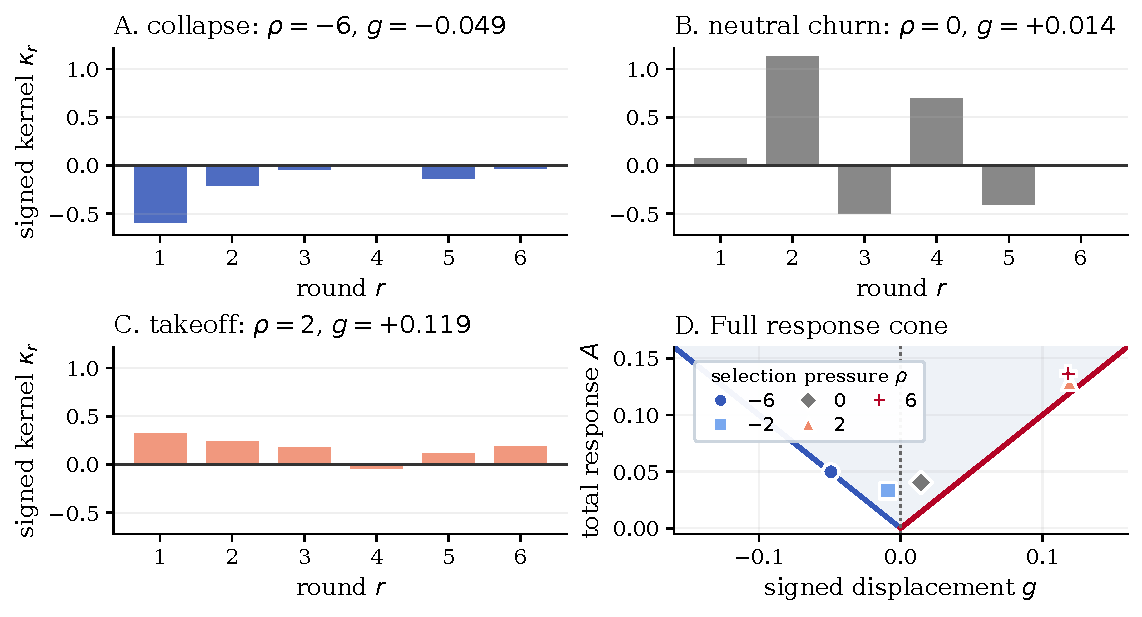
\includegraphics[width=0.84\linewidth]{fig3_takeoff_kernels.pdf}
\caption{Full empirical response geometry. Signed kernels show nearly monotone collapse, alternating neutral churn, and distributed takeoff. In the cone, monotone collapse and takeoff occupy opposite boundary rays; cancellation lifts trajectories into the interior. Cone labels are $\rho$.}
\label{fig:kernels}
\end{figure}

\begin{samepage}
Figure~\ref{fig:kernels} makes the finite-response connection explicit. Collapse hugs the left wall with $E=0.0006$; $\rho=2$ takeoff hugs the right with $E=0.0098$; neutral selection rises into the cone because $64.5\%$ of its motion cancels. The panels expose coherent negative delivery, alternating churn, and coherent positive delivery. Together, these form the discrete counterpart of the entropy paper's causal interior between ideal walls.
\end{samepage}

The geometry yields a compact takeoff diagnostic. For $A>0$, define response efficiency and inheritance lift by
\begin{equation}\label{eq:diagnostic}
\eta(\rho)=\frac{|g(\rho)|}{A(\rho)}=1-\frac{E(\rho)}{A(\rho)},
\qquad
I_6(\rho)=Q_6^{\mathrm{recursive}}(\rho)-Q_6^{\mathrm{restart}}(\rho).
\end{equation}
Then $(g,\eta,I_6)$ separates direction, persistence, and recursive amplification. For $\rho=2$ it is $(0.119,0.924,0.185)$: positive, retained, and amplified by inheritance. The $\rho=-6$ branch has negative gain and $\eta=0.988$, an equally efficient collapse; neutral selection has $\eta=0.355$ and almost no inheritance lift, the signature of churn.

Proposition~\ref{prop:selector} locates the source: child-pool fitness variance is instantaneous susceptibility. Generation replenishes it, selection converts it into drift, and inheritance transports the drift. Population concentration then lowers susceptibility and produces the observed finite plateau.

The study used 7,688 primary and 1,152 matched-control calls; all 9,849 Bedrock calls, including pilots and gates, cost an estimated $1.45$. Primary terminal API failure was $0.052\%$, and scoring was deterministic from hidden references.

Under fixed model weights, one calibrated selector moves recursive physics populations through collapse, neutral churn, and takeoff; inherited self-revision strengthens the improving branch. Weight updates would add a slower recursion. The inference-time kernel is already visible: signed, finite, and experimentally controllable.

\vspace{-0.5em}
\begin{thebibliography}{9}\fontsize{10}{10.8}\selectfont
\setlength{\parskip}{0pt}
\setlength{\itemsep}{-0.10em}
\setlength{\parsep}{0pt}

\bibitem{shumailov2024}
I.~Shumailov, Z.~Shumaylov, Y.~Zhao, et al.
\newblock \href{https://doi.org/10.1038/s41586-024-07566-y}{AI models collapse when trained on recursively generated data}.
\newblock \emph{Nature} 631, 755--759, 2024.

\bibitem{kazdan2025}
J.~Kazdan, R.~Schaeffer, A.~Dey, et al.
\newblock Collapse or thrive: Perils and promises of synthetic data in a self-generating world.
\newblock \emph{ICML}, PMLR 267:29469--29494, 2025.

\bibitem{qiu2025}
S.~Qiu, S.~Guo, Z.-Y. Song, et al.
\newblock \href{https://arxiv.org/abs/2504.16074}{PHYBench: Holistic evaluation of physical perception and reasoning in large language models}.
\newblock arXiv:2504.16074, 2025.

\bibitem{amazonNova}
Amazon Artificial General Intelligence.
\newblock \href{https://arxiv.org/abs/2506.12103}{The Amazon Nova family of models: Technical report and model card}.
\newblock Amazon Technical Reports, 2025.

\bibitem{landersEntropy}
J.~R. Landers.
\newblock The entropy of finite response: Causal kernels, closure, and spread.
\newblock Manuscript, 2026.

\bibitem{landersSpectrum}
J.~R. Landers.
\newblock The response spectrum of recursive self-improvement.
\newblock Manuscript, 2026.

\end{thebibliography}

\end{document}
